%----------------------------------------------------------------------------------------
%	PACKAGES AND OTHER DOCUMENT CONFIGURATIONS
%----------------------------------------------------------------------------------------

\documentclass[twoside,twocolumn,a4paper]{article}

\usepackage{blindtext} % Package to generate dummy text throughout this template 

\usepackage{mhchem}

\usepackage{gensymb}

\usepackage[super]{natbib}

\usepackage[T1]{fontenc} % Use 8-bit encoding that has 256 glyphs

\usepackage{lmodern}

\usepackage[hyphenbreaks]{breakurl}

\usepackage[hyphens]{url}

%\usepackage[super,sort&compress]{natbib}
%\usepackage{natbib}
%\setlength{\bibsep}{0.0pt}

\usepackage{graphicx}

\linespread{1.05} % Line spacing - Palatino needs more space between lines
\usepackage{microtype} % Slightly tweak font spacing for aesthetics

\usepackage[spanish]{babel} % Language hyphenation and typographical rules

\usepackage[numbib,notlof,notlot,nottoc]{tocbibind} % Shows bibliography as a section

\usepackage[hmarginratio=1:1,top=32mm,columnsep=20pt]{geometry} % Document margins

\usepackage[hang, small,labelfont=bf,up,textfont=up]{caption} % Custom captions under/above floats in tables or figures

\usepackage[section]{placeins}

\usepackage{float}

\usepackage{booktabs} % Horizontal rules in tables

\usepackage{enumitem} % Customized lists

\setlist[itemize]{noitemsep} % Make itemize lists more compact

\usepackage{abstract} % Allows abstract customization

\renewcommand{\abstractnamefont}{\normalfont\bfseries} % Set the "Abstract" text to bold

\usepackage{fancyhdr} % Headers and footers
\pagestyle{fancy} % All pages have headers and footers
\fancyhead{} % Blank out the default header
\fancyfoot{} % Blank out the default footer
\fancyhead[C]{Laboratorio 4 $\bullet$ Informe Pr\'actica Especial $\bullet$ Grupo 3: Poggi, R\'ios Ch\'avez} % Custom header text
\fancyfoot[C]{\thepage} % Custom footer text

\usepackage{titling} % Customizing the title section

\usepackage{hyperref} % For hyperlinks in the PDF

%----------------------------------------------------------------------------------------
%	TITLE SECTION
%----------------------------------------------------------------------------------------

\setlength{\droptitle}{-4\baselineskip} % Move the title up

\pretitle{\begin{center}\LARGE\bfseries} % Article title formatting
\posttitle{\end{center}} % Article title closing formatting
\title{Termoelectricidad} % Article title
\author{%
\textsc{Ignacio Poggi} \\[1ex] % Your name
\normalsize \href{mailto:ignaciop.3@gmail.com}{ignaciop.3@gmail.com} % Your email address
\and % Uncomment if 2 authors are required, duplicate these 4 lines if more
\textsc{Carlos R\'ios Ch\'avez} \\[1ex] % Second author's name
\normalsize \href{mailto:carlos_rios_ch@hotmail.com}{carlos\_rios\_ch@hotmail.com} % Second author's email address
}



\date{Grupo 3 - Laboratorio 4, C\'atedra Schmiegelow - Departamento de F\'isica, Facultad de Ciencias Exactas y Naturales, Universidad de Buenos Aires \newline \\ \today} % Leave empty to omit a date
\renewcommand{\maketitlehookd}{%
\begin{abstract}
\noindent En este trabajo se realiz\'o la caracterizaci\'on de una celda Peltier midiendo el coeficiente de Seebeck $\alpha$, resistencia $R$ y conductividad t\'ermica $K$; a trav\'es de los datos obtenidos de la diferencia de temperatura, voltaje y corriente circundante entre sus dos caras. Finalmente se obtuvo el rendimiento de la celda y se compar\'o con el de otras m\'aquinas t\'ermicas.
\end{abstract}
}

%----------------------------------------------------------------------------------------

\begin{document}
\maketitle

% Print the title

%----------------------------------------------------------------------------------------
%	ARTICLE CONTENTS
%----------------------------------------------------------------------------------------

\section{Introducci\'on}


Se denomina termoelectricidad a un conjunto de efectos o fen\'omenos f\'isicos que relacionan a la termodin\'amica con la electricidad. En equilibrio termodin\'amico, los portadores de carga en un conductor pueden generar un flujo de calor, pudiendo transformar energ\'ia mec\'anica en energ\'ia t\'ermica y viceversa. Entre estos fen\'omenos, podemos destacar el efecto Seebeck, Peltier y Joule.

\subsection{Efecto Seebeck}

Si se tiene un circuito formado por dos metales distintos, $A$ y $B$, con dos uniones a diferente temperatura, $T$ y $T + \Delta T$, se establece un flujo de corriente el\'ectrica debido a que los portadores de carga difunden en contra del gradiente de temperatura. Esto produce acumulaci\'on de carga en el extremo fr\'io y un vaciamiento del extremo caliente del termopar. Este desbalance de portadores genera un campo el\'ectrico, que a su vez origina una fuerza termoelectromotriz $\epsilon_{AB}$, que depende de los metales utilizados en la uni\'on y de la diferencia de temperatura entre las dos uniones.\newline

\par
Se puede definir al coeficiente Seebeck $\alpha_{AB}$ como la relaci\'on entre $\epsilon_{AB}$ y $T$, de la siguiente manera:

\begin{equation}
\label{eq:seebeck}
\alpha_{AB} = \frac{d\epsilon_{AB}}{dT}
\end{equation}

La ecuaci\'on (\ref{eq:seebeck}) puede definirse macrosc\'opicamente como:

\begin{equation}
\label{eq:seebeck2}
\alpha_{AB} = \frac{\Delta V}{\Delta T}
\end{equation}

donde $\Delta V$ y $\Delta T$ son las diferencia de potencial neta  y temperatura entre los metales $A$ y $B$, respectivamente.

\subsection{Efecto Peltier}

Rec\'iprocamente al efecto Seebeck, al circular una corriente el\'ectrica $I$ por la uni\'on entre distintos materiales, se produce una transferencia de calor, como se esquematiza en la Figura \ref{fig:peltier}. La potencia calor\'ifica intercambiada en la uni\'on entre los puntos $A$ y $B$ es:

\begin{equation}
\label{eq:peltier}
\dot{Q} = J\Delta T \alpha_{AB} = J \pi_{AB}
\end{equation}

siendo $\pi_{AB}$ el coeficiente Peltier (calor intercambiado en la uni\'on por unidad de tiempo y de corriente que circula por la misma), $J$ el flujo de corriente el\'ectrica, $\Delta T$ la diferencia de temperatura entre los puntos $A$ y $B$, y $\alpha_{AB}$ el coeficiente Seebeck.


\begin{figure}[H]
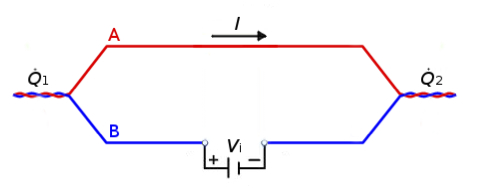
\includegraphics[width=\linewidth]{peltier.jpg}
\caption{Esquema de un circuito formado por los materiales A y B con dos uniones. La circulaci\'on de corriente origina un flujo de calor, produciendo el efecto Peltier.}
\label{fig:peltier}
\end{figure}

\subsection{Efecto Joule}

Para una caracterizaci\'on completa de la celda, se deben tener en cuenta la difusi\'on de calor a trav\'es de la misma debido al gradiente de temperatura, y la disipaci\'on por efecto Joule.\newline

\par
La difusion de calor del lado mas caliente al fr\'io por unidad de tiempo para cada elemento esta dado por la ley de Fourier:

\begin{equation}
\label{eq:calor}
\dot{Q}_{Fourier} = -k \frac{A}{L} \Delta T
\end{equation}

donde $k$ es el coeficiente de conductividad t\'ermica de cada elemento por unidad de longitud, $A$ el \'area, $l$ la longitud de cada elemento y $\Delta T$ la diferencia de temperatura en los extremos (el signo negativo indica que el calor fluye en contra del gradiente de temperatura).\newline

\par
El efecto Joule est\'a representado por la transformaci\'on de trabajo el\'ectrico en calor, debido a la resistencia $R$ del circuito. La p\'erdida de energ\'ia asociada es:

\begin{equation}
\label{eq:joule}
\dot{Q}_{Joule} = I^{2}R = I^{2}\rho \frac{L}{A}
\end{equation}

donde $\rho$ es la resistividad el\'ectrica del conductor respectivamente.


\subsection{Celdas termoel\'ectricas}

Una celda Peltier est\'a compuesta por un cierto n\'umero de termopares (pares de semiconductores de tipo N y P), conectados en serie con las uniones ubicadas alternadamente sobre las dos caras. Dichas caras est\'an recubiertas de un material cer\'amico, para mejorar la disipaci\'on del calor, como muestra la Figura \ref{fig:celda}.

\begin{figure}[H]
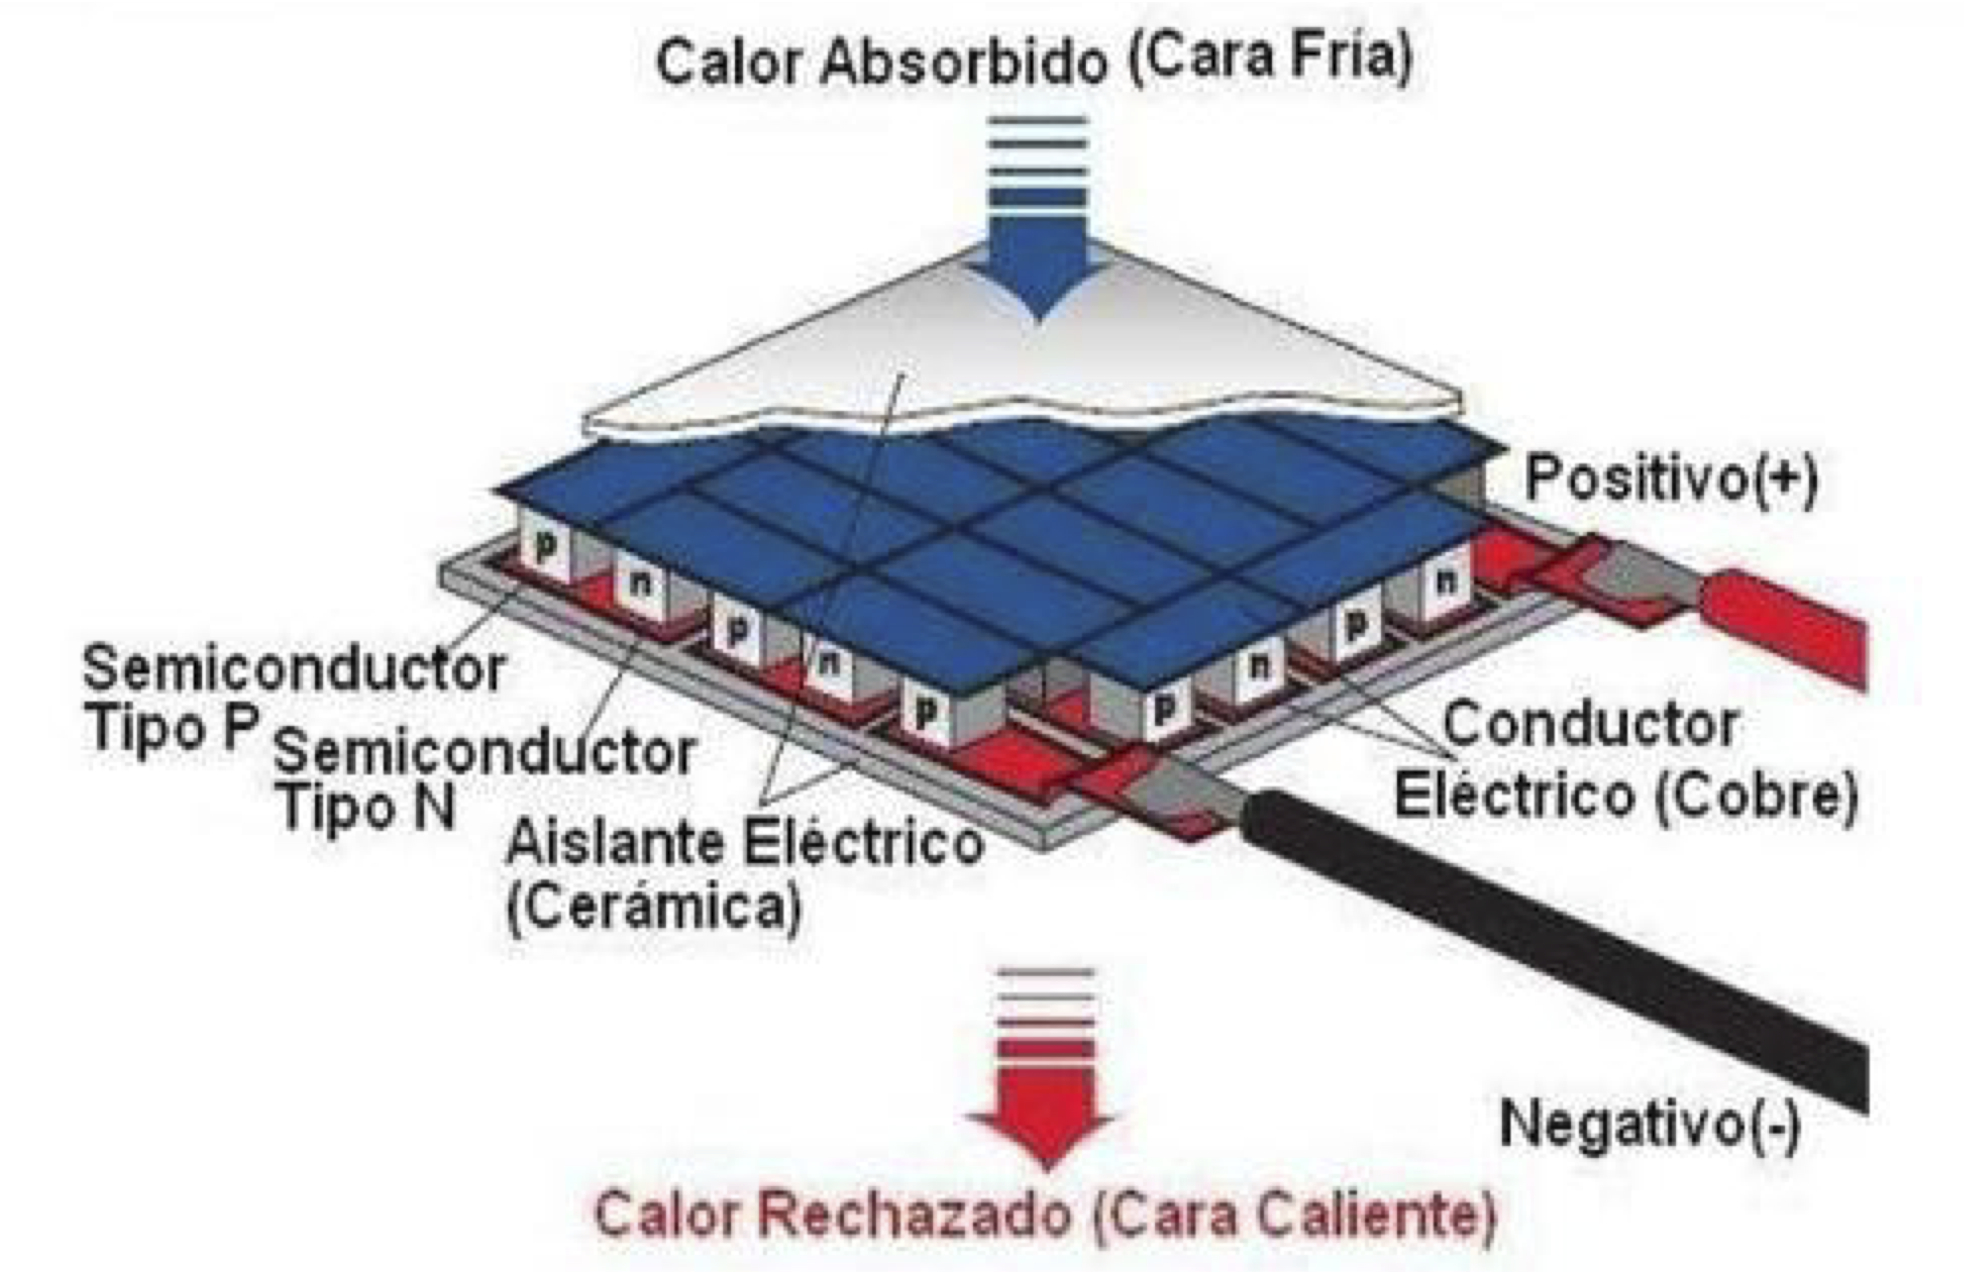
\includegraphics[width=\linewidth]{celda.jpg}
\caption{Esquema de una celda Peltier. Se observan los componentes semiconductores en el interior de la misma y las caras cer\'amicas a distinta temperatura.}
\label{fig:celda}
\end{figure}

Si ambas caras de la celda se encuentran en contacto con reservorios a distintas temperaturas, se manifiesta el efecto Seebeck, por lo tanto puede ser utilizada como generador de electricidad. An\'alogamente, al hacer pasar una corriente $I$ por la misma, las uniones sobre una de las caras absorber\'an y las contrarias liberar\'an calor (efecto Peltier), operando como una m\'aquina frigor\'ifica o una fuente de calor.

Por \'ultimo, para calcular el rendimiento de la celda como maquina termica, utilizando las ecuaciones (\ref{eq:peltier}) y (\ref{eq:joule}) se obtiene que el calor intercambiado en cada una de las caras (en r\'egimen estacionario) es:

\begin{equation}
\label{eq:qcaras}
\dot{Q_{i}} = \pm I\alpha T_{i} - K(T_{i} - T_{j}) + \frac{I^{2}R}{2}
\end{equation}


donde $\alpha$ y $K$ contienen la contribuci\'on de todos los elementos conductores al efecto Peltier y a la difusi\'on de calor, y $i = \{1,2\}$. De la misma forma, la potencia el\'ectrica aplicada esta dada por la siguiente ecuaci\'on:

\begin{equation}
\label{eq:potencia}
\dot{W} = VI = I \alpha \Delta T + I^{2}R
\end{equation}

Mediante las ecuaciones (\ref{eq:qcaras}) y (\ref{eq:potencia}), se puede obtener la eficiencia y el rendimiento de la celda como m\'aquina t\'ermica con las siguientes expresiones:


\begin{equation}
\label{eq:eficiencia}
\eta = \frac{-\dot{W}}{-\dot{Q_{c}}}
\end{equation}

\begin{equation}
\label{eq:rendimiento}
COP = \frac{-\dot{Q_{f}}}{+\dot{W}}
\end{equation}

siendo $\dot{Q_{f}}$ y $\dot{Q_{c}}$ el calor intercambiado por la cara fria y caliente, respectivamente.



%------------------------------------------------

\section{Dispositivo experimental}

Los instrumentos de laboratorio utilizados fueron:
\begin{itemize}
\item PC con software MATLAB para la adquisici\'on y an\'alisis de los datos.
\item Placa de adquisici\'on de datos National Instruments NI-USB 6120.
\item Celda Peltier Marlow Industries DT3-6.
\item Dos sensores de temperatura LM35.
\item Generador de corriente continua LG GP4303D.
\item Unidad de medici\'on de corriente/voltaje Agilent B2901A.
\item Cables Banana-Banana y Banana-Cocodrilo.
\end{itemize}





En esta experiencia, se trabaj\'o con un cristal piezoel\'ectrico de base cuadrada, cortado a +5 \degree respecto de uno de sus ejes; contenido en una base cerrada de acr\'ilico. En dos de las caras del cristal, se encontraban dispuestos electrodos de metal, cada uno con un alambre soldado, cada uno de los cuales estaban en serie con una resistencia de 10 K$\Omega$. En la siguiente figura se puede ver un esquema del dispositivo utilizado:

\begin{figure}[H]
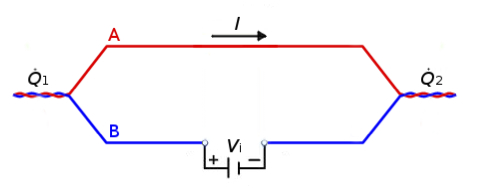
\includegraphics[width=\linewidth]{peltier.jpg}
\caption{Esquema del dispositivo experimental utilizado. .}
\label{fig:dispexp}
\end{figure}

En uno de los alambres mencionados, se utiliz\'o el generador de funciones para aplicar una se\~nal de entrada $V_{1}$ de amplitud 2 Vpp y frecuencia variable. Luego, sobre el otro alambre se registr\'o la se\~nal de salida $V_{2}$, en primera instancia con el osciloscopio y luego con el amplificador lock-in. Con \'este \'ultimo tambi\'en se obtuvo la diferencia de fase entre la se\~nal de entrada y la de salida. Cabe aclarar que, para poder establecer una se\~nal de referencia requerida por el amplificador lock-in, se conecto una de las salidas del generador de funciones con la entrada de referencia del amplificador.


Finalmente, se conectaron el osciloscopio (mediante cable USB) y el amplificador (mediante interfaz GPIB) a una PC con software MATLAB,    con el cual se ejecut\'o un script para poder recolectar y analizar los datos enviados por los equipos mencionados.

%------------------------------------------------
\section{Resultados y an\'alisis}

Para poder estimar la frecuencia de resonancia del cristal de cuarzo, en primer lugar se utiliz\'o el generador de funciones para realizar manualmente un barrido de frecuencias y el osciloscopio para poder visualizar la amplitud de la onda y obtener la campana de resonancia de dicho cristal, como muestra la siguiente figura:

\begin{figure}[H]
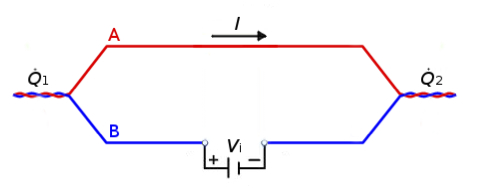
\includegraphics[width=\linewidth]{peltier.jpg}
\caption{Campana de resonancia obtenida mediante un barrido de frecuencias manual con el osciloscopio.}
\label{fig:detallecampanaOSC}
\end{figure}

Luego, se pudo calcular la frecuencia de resonancia y el ancho de la campana, dando como resultado $\omega_{r}$ = (50108 $\pm$ 7) Hz y $\Delta \omega$ = (6,15 $\pm$ 0,10) Hz respectivamente. Con estos datos, se obtuvo el factor de m\'erito del circuito, $Q$ = 8147 $\pm$ 70. \newline

\par
Adem\'as, se intent\'o calcular la frecuencia de antirresonancia utilizando este m\'etodo; pero al aumentar la escala en el gr\'afico anterior en la zona correspondiente a dicha frecuencia (50,025 kHz $< \omega_{a} <$ 50,03 kHz), notamos que por la baja resoluci\'on del osciloscopio no se pudo obtener un valor confiable para $\omega_{a}$. \newline


\par
Posteriormente se analizaron los datos obtenidos por el amplificador lock-in. Se realizaron varios barridos de frecuencia con distintos niveles de resoluci\'on en la variaci\'on de la frecuencia, procurando que el barrido sea fino en los rangos que m\'as nos interesaron, es decir cerca a la resonancia y la antirresonancia, previamente estimadas. Se trabaj\'o con todas las mediciones en una sola base de datos y para determinar la frecuencia de resonancia se utilizaron tres m\'etodos, el primero consisti\'o en ajustar la curva de voltaje a una curva lorentziana, ajuste del cual se obtuvo que $\omega_{r}$ = (50097,85 $\pm$ 0,01) Hz (la bondad del ajuste fue $R^{2}$ = 0,992), como muestra la Figura \ref{fig:ajuste}:


\begin{figure}[H]
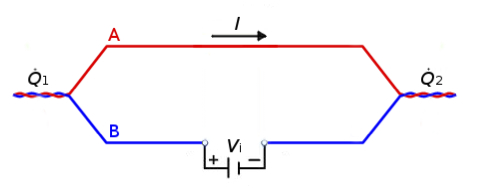
\includegraphics[width=\linewidth]{peltier.jpg}
\caption{Ajuste a una funci\'on lorentziana del voltaje con respecto a la frecuencia.}
\label{fig:ajuste}
\end{figure}


El segundo m\'etodo consisti\'o en encontrar la frecuencia para la cual la transferencia de energ\'ia es m\'axima considerando que la transferencia es directamente proporcional al voltaje registrado,  Figura \ref{fig:detalleRESamp}. Se obtuvo que $\omega_{r}$ = (50097,9 $\pm$ 0,3) Hz y en el caso de la antirresonancia se determin\'o la frecuencia en la cual la transferencia de energ\'ia es m\'inima, obteni\'endose que $\omega_{a}$ = (50284,4 $\pm$ 0,3) Hz, Figura \ref{fig:detalleANTamp}.


\begin{figure}[H]
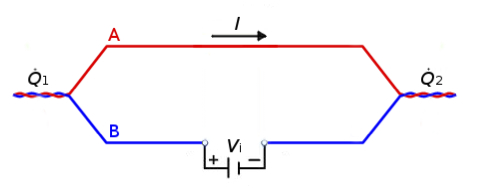
\includegraphics[width=\linewidth]{peltier.jpg}
\caption{Detalle de la campana de resonancia, donde la l\'inea punteada indica el voltaje m\'aximo y la l\'inea horizontal indica los puntos para los cuales el voltaje m\'aximo se reduce a la mitad.}
\label{fig:detalleRESamp}
\end{figure}


\begin{figure}[H]
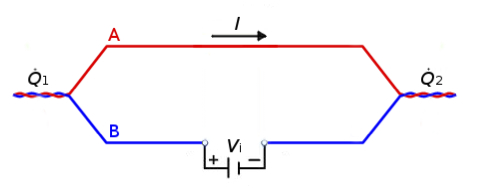
\includegraphics[width=\linewidth]{peltier.jpg}
\caption{Detalle del intervalo donde se produce la antirresonancia indicada por la l\'inea punteada.}
\label{fig:detalleANTamp}
\end{figure}

El \'ultimo m\'etodo que utilizamos consisti\'o en analizar la fase en funci\'on de la frecuencia, considerando que cuando la fase llega a cero de forma descendente corresponde a la fase en la frecuencia de resonancia y que cuando la fase pasa por cero de forma ascendente es que corresponde a la frecuencia de antirresonancia. Se obtuvo que la frecuencia de resonancia es $\omega_{r}$ = (50097,25 $\pm$ 0,05) Hz y que $\omega_{a}$ = (50284,65 $\pm$ 0,05) Hz, en la Figura \ref{fig:fase} se ve la curva completa mientras que en las Figuras \ref{fig:bajada} y \ref{fig:subida} se ven en detalle los puntos donde la diferencia de fase pasa por cero. 

\begin{figure}[H]
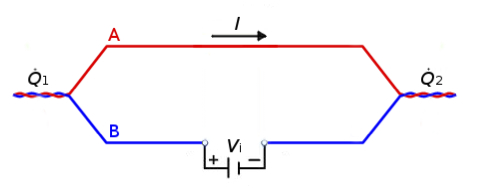
\includegraphics[width=\linewidth]{peltier.jpg}
\caption{Diferencia de fase entre la se\~nal de entrada al piezoel\'ectrico y la se\~nal de salida con respecto a la frecuencia.}
\label{fig:fase}
\end{figure}

\begin{figure}[H]
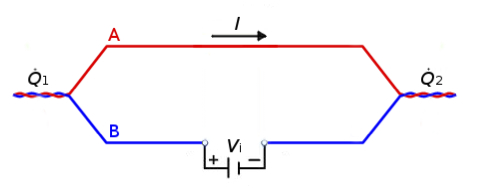
\includegraphics[width=\linewidth]{peltier.jpg}
\caption{Detalle de la diferencia de fase en el intervalo donde se produce la resonancia indicada por la l\'inea punteada.}
\label{fig:bajada}
\end{figure}

\begin{figure}[H]
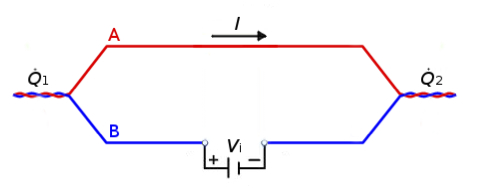
\includegraphics[width=\linewidth]{peltier.jpg}
\caption{Detalle de la diferencia de fase en el intervalo donde se produce la antirresonancia indicada por la l\'inea punteada.}
\label{fig:subida}
\end{figure}

Para obtener $\Delta \omega$ se calcularon las frecuencias para las cuales la amplitud m\'axima se habia reducido a la mitad, figura \ref{fig:detalleRESamp}, eso nos di\'o una idea del ancho de la campana $\Delta \omega$ = (5,90 $\pm$ 0,01) Hz. Si comparamos el valor de la frecuencia de resonancia con el ancho de la campana obtenemos el factor de m\'erito, el cual cuanto m\'as grande es, nos indica que m\'as aguda es la campana y que por lo tanto el material es m\'as \'util como resonador en una frecuencia espec\'ifica; en este caso se encontr\'o que el factor de m\'erito es $Q$ = 8491 $\pm$ 5.

Los par\'ametros del circuito que modela el comportamiento del piezoel\'ectrico fueron determinados mediante las ecuaciones (\ref{eq:transferenciar}), (\ref{eq:merito}), (\ref{eq:wr}) y (\ref{eq:wa}), obteni\'endose que la resistencia es $R$ = (13,65 $\pm$ 0,09) K$\Omega$, la inductividad $L$ = (3161 $\pm$ 5) H, la capacitancia es $C$ = (0,126 $\pm$ 0,004) pF; y que la capacitancia producida por la capa de oro que envuelve al piezoel\'ectrico es de $C_{2}$ = (16,9 $\pm$ 0,5) pF.

%------------------------------------------------

\section{Conclusiones}

Se puede observar que los distintos m\'etodos para determinar la frecuencia de resonancia var\'ian en d\'ecimas de Hz, por lo cual consideramos que la experiencia tuvo bastante precisi\'on pues se trabaj\'o con frecuencias del \'orden de los kHz; incluso en un primer barrido manual con el osciloscopio. \\

Sobre la frecuencia de antirresonancia pudimos notar que es preciso un instrumento lo bastante sensible como para poder determinarla, pues el barrido que se realiz\'o con el osciloscopio registraba bastante ruido por lo que no se pudo trabajar con esos datos para determinar dicha frecuencia, mientras que con los datos obtenidos con el amplificador lock-in se pudo obtener un perfil de la curva de voltaje mucho m\'as limpio en comparaci\'on al del osciloscopio y m\'as aun tomando en cuenta el registro de la diferencia de fase que nos permiti\'o el amplificador. \\

El alto factor de m\'erito que obtuvimos nos indica que la campana es bastante aguda, es decir que el ancho de la campana es peque\~no en comparaci\'on a la altura; por lo cual concluimos que el ancho de banda en el cual resuena material piezoel\'ectrico es m\'as estrecho, o visto de otra manera, posee una baja tasa de p\'erdida de energ\'ia en relaci\'on a la almacenada por el mismo.

%----------------------------------------------------------------------------------------
%	REFERENCE LIST
%----------------------------------------------------------------------------------------
\newpage
\begin{thebibliography}{99} % Bibliography - this is intentionally simple in this template


\bibitem{eq:oderlc} R. K. Nagle, E. B. Saff, A. D. Snider, \textit{Ecuaciones diferenciales y problemas con valores en la frontera}, $4^{ta}$ edici\'on, Pearson Educaci\'on M\'exico, 2005, p\'ag. 285
\bibitem{eq:props} http://materias.df.uba.ar/labo4Ba2016c1/files/2014/03/Piezo.pdf 
 
\end{thebibliography}


%----------------------------------------------------------------------------------------

\end{document}